
\chapter{Introduction to parsing}

Parsing is a fundamental activity in many programs, and for all but the most trivial cases, it is a challenging topic.
Parsing is often done when we need to read data that is stored in a custom format so that we can process it or perform queries on it.
Or we may be required to parse a DSL (Domain-Specific Language)—these are mini task-specific languages that appear to be growing in popularity.
Whether we need to read data in a custom format or code written using a DSL, we will need to create a suitable parser.
This can be done by handcrafting, or by using one of Python’s generic parsing modules.



Fortunately, for some data formats, we don't have to write a parse at all.


In fact, Python has built-in support for reading and writing a wide range of data formats, including:
\begin{itemize}
\item delimiter-separated data with the \verb|csv| module
\item Windows-style \verb|.ini| files with the \verb|configparse| module
\item JSON data with the \verb|json| module
\item ... 
\end{itemize}


\keyword{In general, if Python already has a suitable parser in the standard library, or as a third-party add-on, it is usually best to use it rather than to write our own.}


\keyword{When it comes to parsing data formats or DSLs for which no parse is available, rather than handcrafting a parser, we can use one of Python's third-party general-purpose parsing modules.}


\section{BNF syntax and parsing terminology}

Parsing is a means of transforming data that is in some structured format into a representation that reflects the data's structure and that can be used to infer the meaning that the data represents.
The parsing process is most often done in two phases:
\begin{enumerate}
\item lexing (also called lexical analysis, tokenizing, or scanning)
\item parsing proper (also called syntactic analysis)
\end{enumerate}


The lexing phase is used to convert the data into a stream of tokens.
In typical cases, each token holds at least two pieces of information:
the token's type (the kind of data or language construct being represented), and
the token's value (which may be empty if the type stands for itself -- for example, a keyword in a programming language).



The parsing phase is where a parser reads each token and performs some semantic action.
The parser operates according to predefined set of grammer rules that define the syntax that the data is expected to follow.
In multiphase parsers, the semantic action consists of building up an internal representation of the input into memory (called an Abstract Syntax Tree -- AST), which serves an input to the next phase.
Once the AST has been constructed, it can be traversed, for example, to query the data, or to write the data out in a different format, or to perform computations that correspond to the meaning encoded in the data.



Data formats and DSLs (Domain-Specific Language) (and programming languages generally) can be described using a \keyword{grammer} -- a set of syntax rules that define what is valid syntax for the data or language.
Of course, just because a statement is syntactically valid doesn't mean that it makes sense.
Nonetheless, being able to define the grammer is very useful, so much so that there is commonly used syntax for describing grammers -- BNF (Backus-Naur Form).
Creating a BNF is the first step to creating a parser, and although not formally necessary, for all but the most trivial grammars it should be considered essential.


\begin{tcolorbox}
In computer science, Backus–Naur form or Backus normal form (BNF) is a metasyntax notation for context-free grammars, often used to describe the syntax of languages used in computing, such as computer programming languages, document formats, instruction sets and communication protocols.   
\end{tcolorbox}




In a BNF there are two kinds of items: terminals and nonterminals.
A terminal is an item which is in its final form, for example, a literal number or string.
A nonterminal is an item that is defined in terms of zero or more other items (which themselves may be terminals or nonterminals).
Every nonterminal must ultimately be defined in terms of zero or more terminals.

Figure \ref{fig:bnf-attributes} shows an example BNF that defines the syntax of a file of ``attributes'', to put things into perspective.

\begin{figure}[!ht]
  \centering
  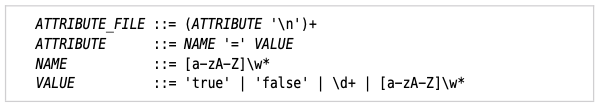
\includegraphics[width=\textwidth]{pics/a-bnf-for-a-file-of-attributes}
  \caption{A BNF for a file of attributes}
  \label{fig:bnf-attributes}
\end{figure}


The symbol \verb|::=| means \keyword{is defined as}.
Nonterminals are written in uppercase italics (e.g., VALUE).
Terminals are either literal strings enclosed in quotes or regular expressions.
The definitions (on the right of the \verb|::=|) are made up of one or more terminals or nonterminals -- these must be encountered in the sequence given to meet the definition.




The BNF in Figure \ref{bnf-arithmetic} defines the four basic arithmetic operations over itegers, as well as parenthesized subexpressions, and all with the correct precedences and (left to right) associativies.
\begin{figure}[!ht]
  \centering
  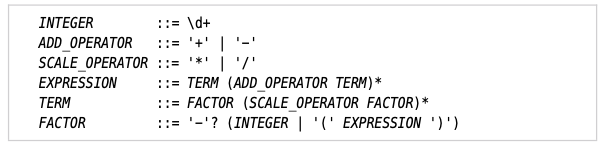
\includegraphics[width=\textwidth]{pics/bnf-arithmetic}
  \caption{A BNF for arithmetic operations}
  \label{fig:bnf-arithmetic}
\end{figure}

\section{Parsing manners}

Typically, there are two manners when no suitable parser can be used directly.
\begin{enumerate}
\item write handcraftd parser
\item write parser with general parser
\end{enumerate}



